\begin{figure}
\centering
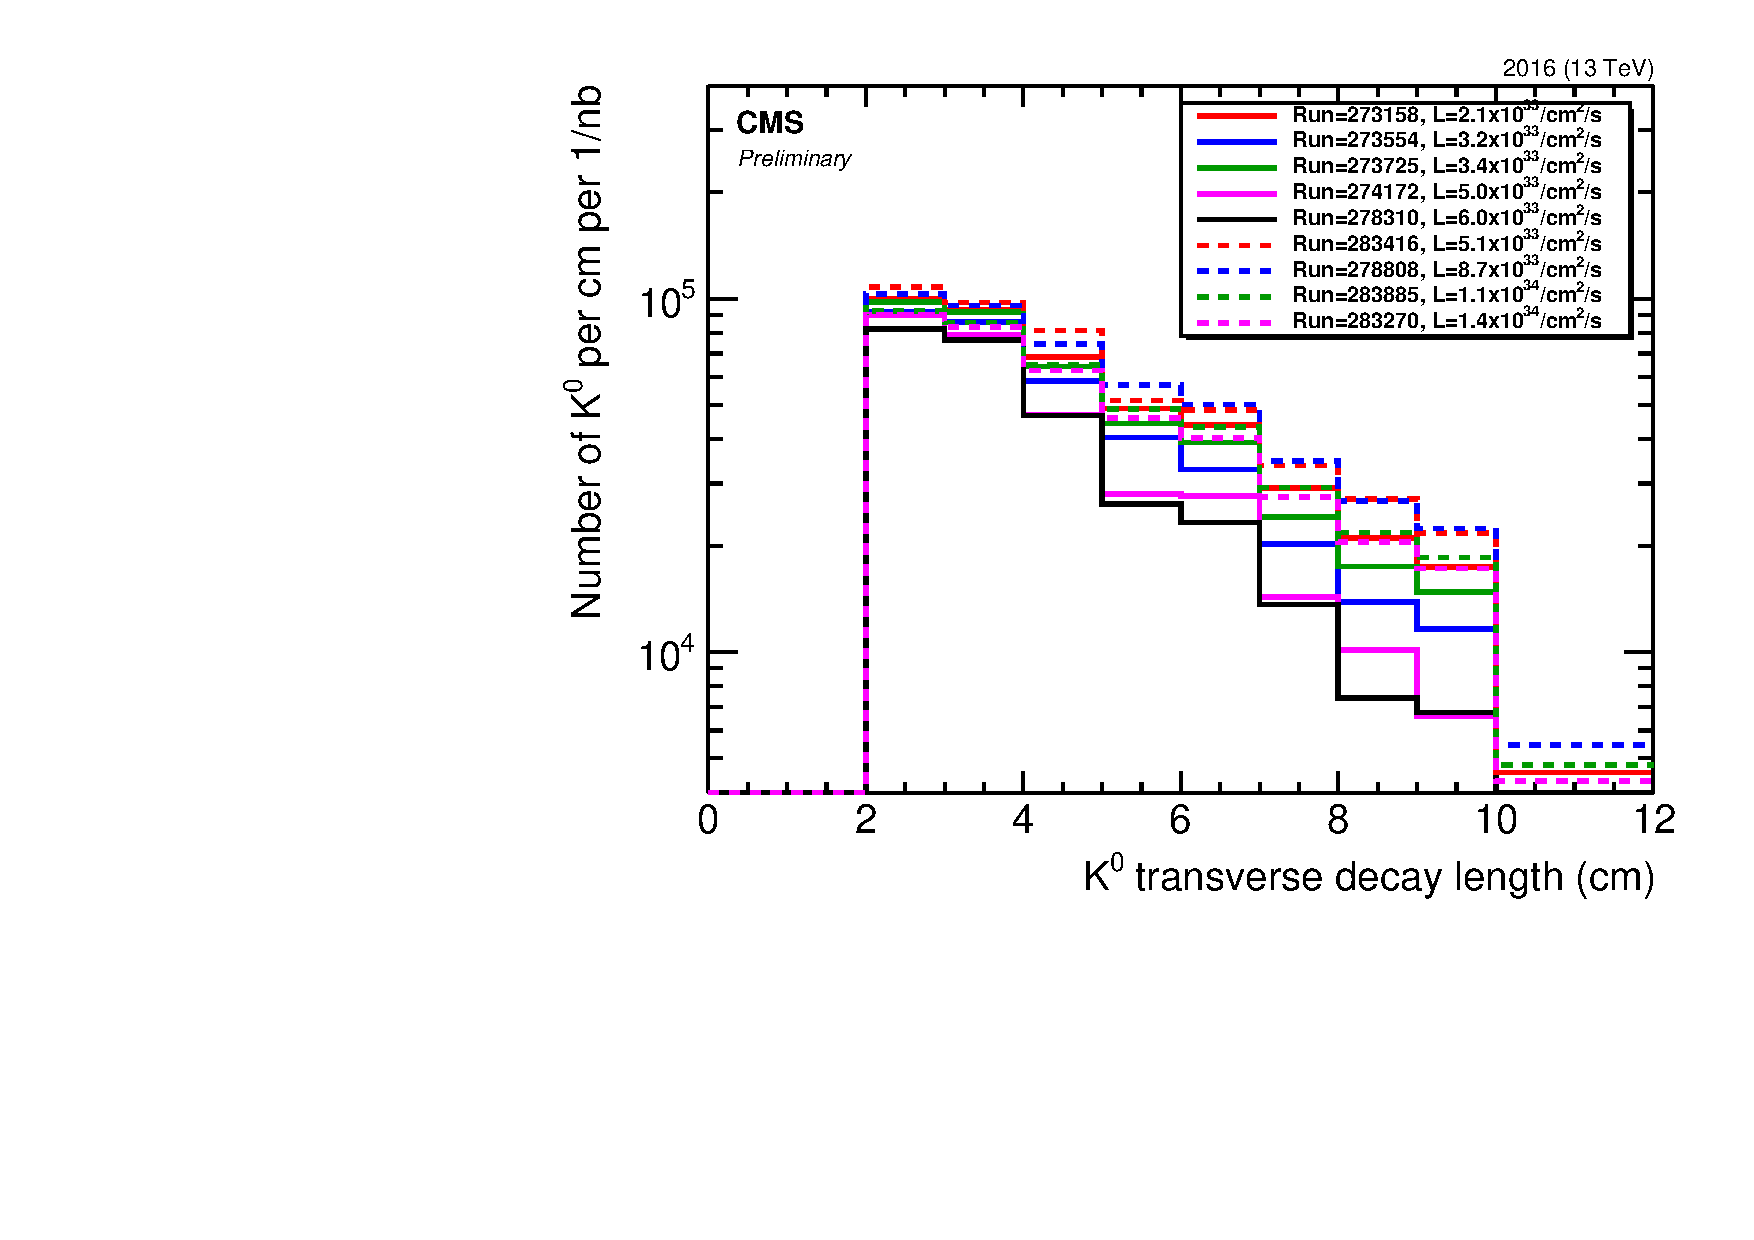
\includegraphics[width=0.45\textwidth]{figures/tracking_eff/2016/k0.pdf}
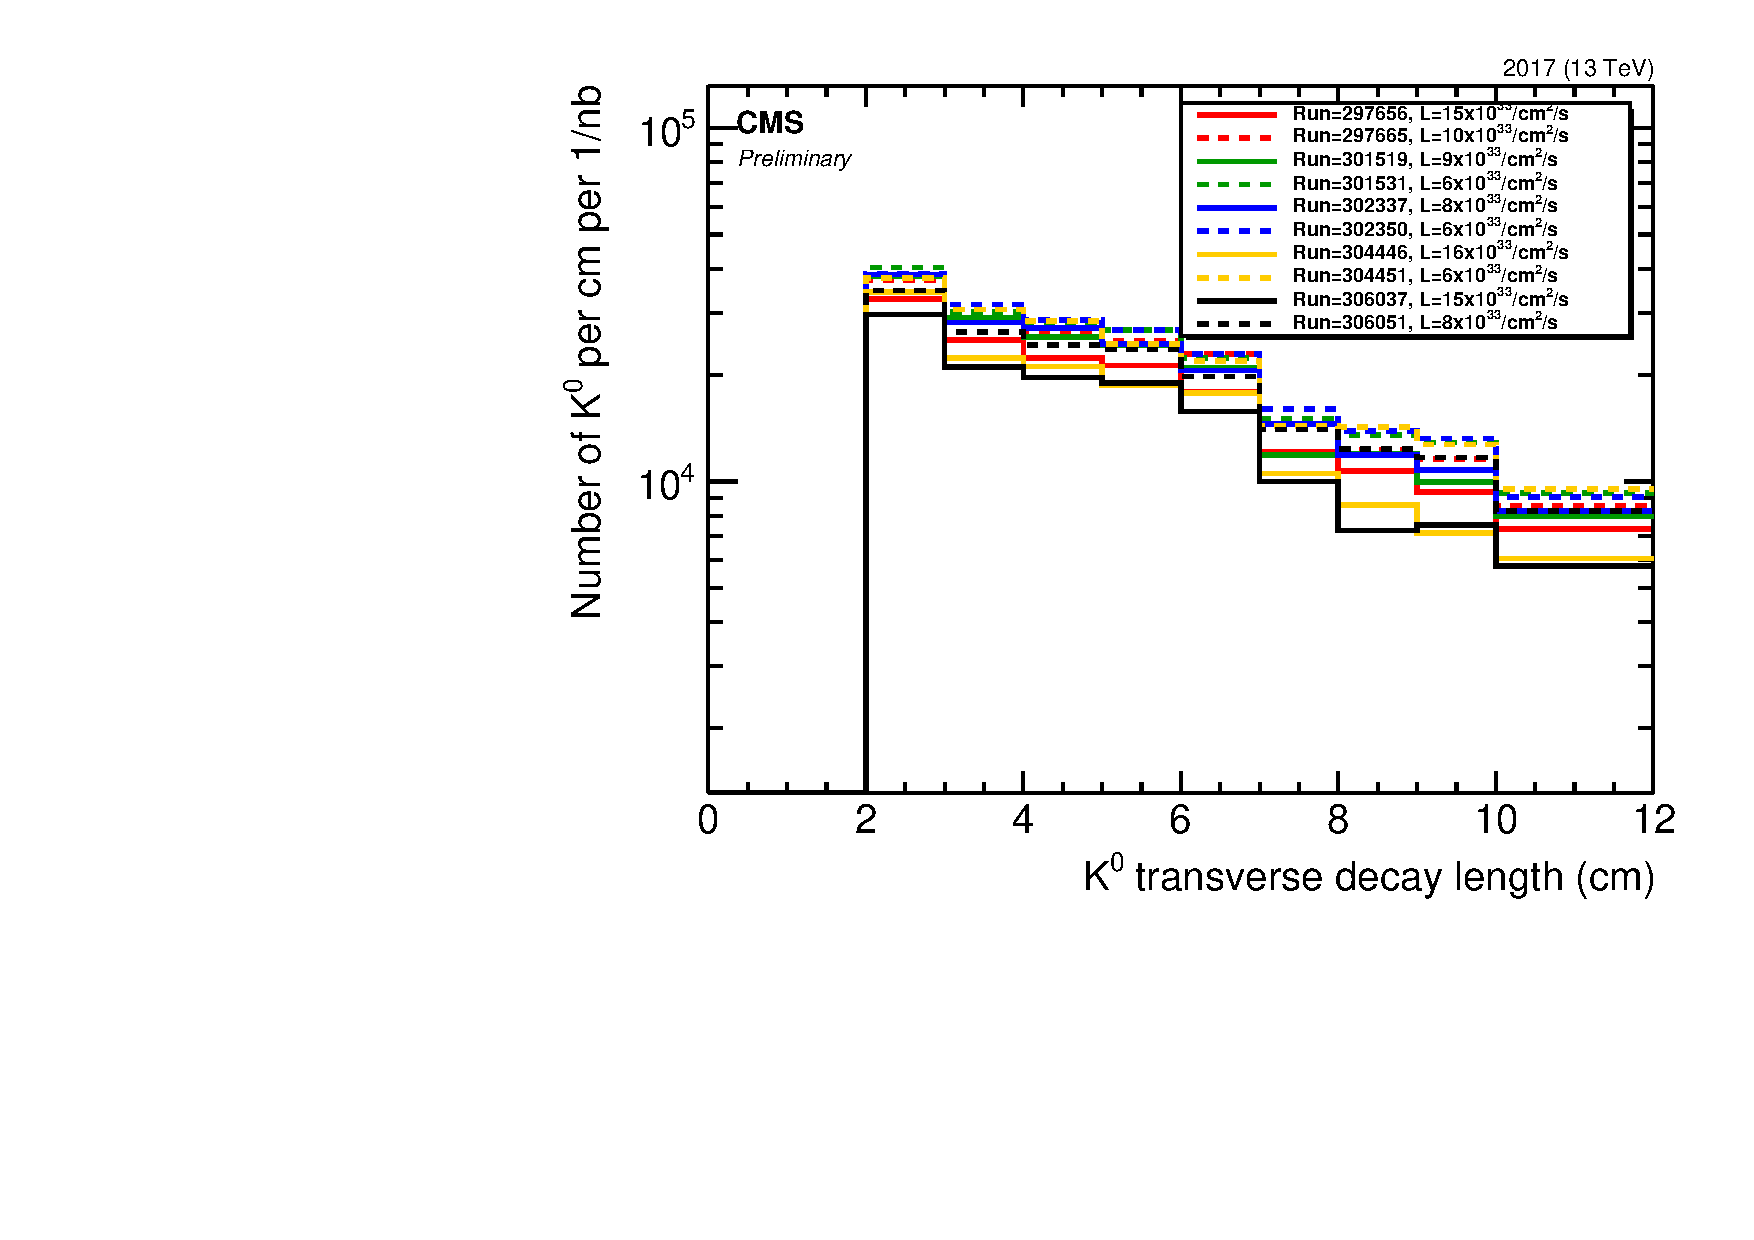
\includegraphics[width=0.45\textwidth]{figures/tracking_eff/2017/k0.pdf}
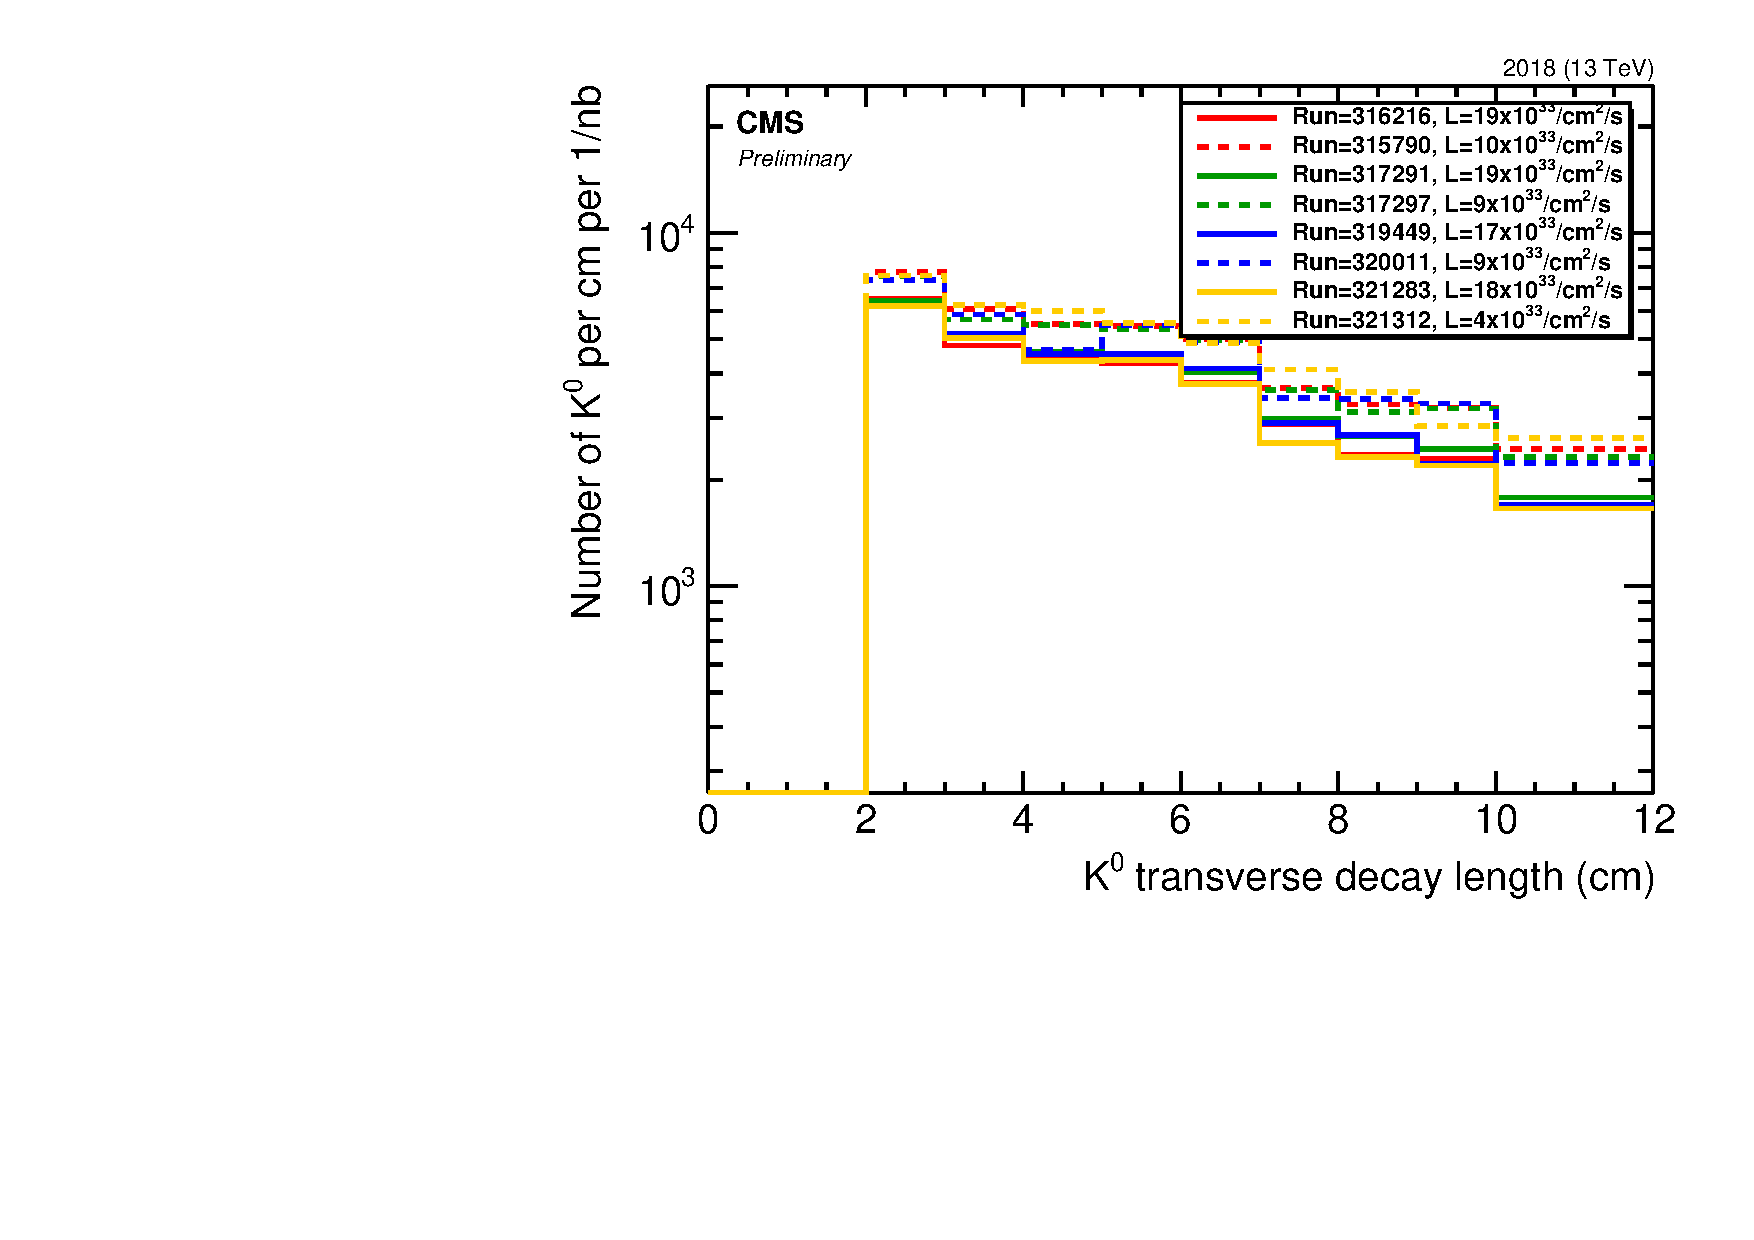
\includegraphics[width=0.45\textwidth]{figures/tracking_eff/2018/k0.pdf}
\caption{Transverse decay length distribution of reconstructed $\Kzero\to\pi^+\pi^-$ candidates for various runs in 2016 (top left), 2017 (top right) and 2018 (bottom). The peak instantaneous luminosity of each run is indicated in the legend, and each distribution is normalized to the integrated luminosity of the run. In the 2016 plot, runs taken before (after) the APV25 saturation effect was mitigated are shown by solid (dashed) lines. In the 2017 plot, the run with lowest (highest) instantaneous luminosity examined in each data-taking era is plotted with a dashed (solid) line. Towards the end of 2017 (orange and black lines) the LHC ran with approximately 20\% fewer proton bunches, meaning that the instantaneous luminosity per bunch crossing was higher than one might naively expect from the instantaneous luminosities shown in the legend.}
\label{k0_tracking_eff}
\end{figure}